\chapter{Growth-Geometry Split in DES-Y3}
Parameter splitting is a common method used to attempt to resolve the tensions discussed in the previous chapter. The idea is to split a parameter and choose analysis settings that restrict each split parameter to describe specific cosmological effects. One of these splits is a growth-geometry split, where we split the relative matter density $\Omega_m$ and the dark energy equation of state $w$ into two parameters. The growth parameter is designed to describe the late-time growth of structure and the geometry parameter designed to describe the background evolution. After splitting the parameters, one can do an analysis to determine how the tension changes and if the split parameters have distinct values from each other. This chapter describes the growth geometry split in $\Omega_m$ and $w$ in DES-Y1~\cite{muir_y1_2021} and DES-Y3. These results are also available in a paper written by Kunhao Zhong, another Masters student, and myself, on arXiv~\cite{zhong_growth_2023} and are pending publication to Physical Review.
\section{Split Matter Power Spectrum}
Since the matter density $\Omega_m$ is split into two parameters, $\Omega_m^{\text{growth}}$ and $\Omega_m^{\text{geo}}$, single growth factor and a single matter power spectrum; these are split as well. From equation (eq), the linear matter power spectrum is proportional to the square of the linear growth factor $D_+(z(a)) = G(z)/(1+z)$, so the growth and geometry power spectra are related by
\begin{equation}
	P^L_{\text{split}}(k,z) = P^L_{\text{geo}}(k,z) \left(\frac{G_{\text{growth}}(z)}{G_{\text{geo}}(z)}\right)^2
\end{equation}
which means $\sigma_8$ is also split according to
\begin{equation}
	\sigma_{8,\text{split}}^2 = \sigma_{8,\text{geo}}^2 \left(\frac{G_{\text{growth}}(z)}{G_{\text{geo}}(z)}\right)^2
\end{equation}
In this analysis, however, we want to go beyond linear scales. To do this, we use the Euclid Emulator to emulate the non-linear matter power spectrum by computing a boost factor
\begin{equation}
	P(k,z) = P^L(k,z) \times B(k,z)
\end{equation}
\begin{figure}[ht]
	\centering
	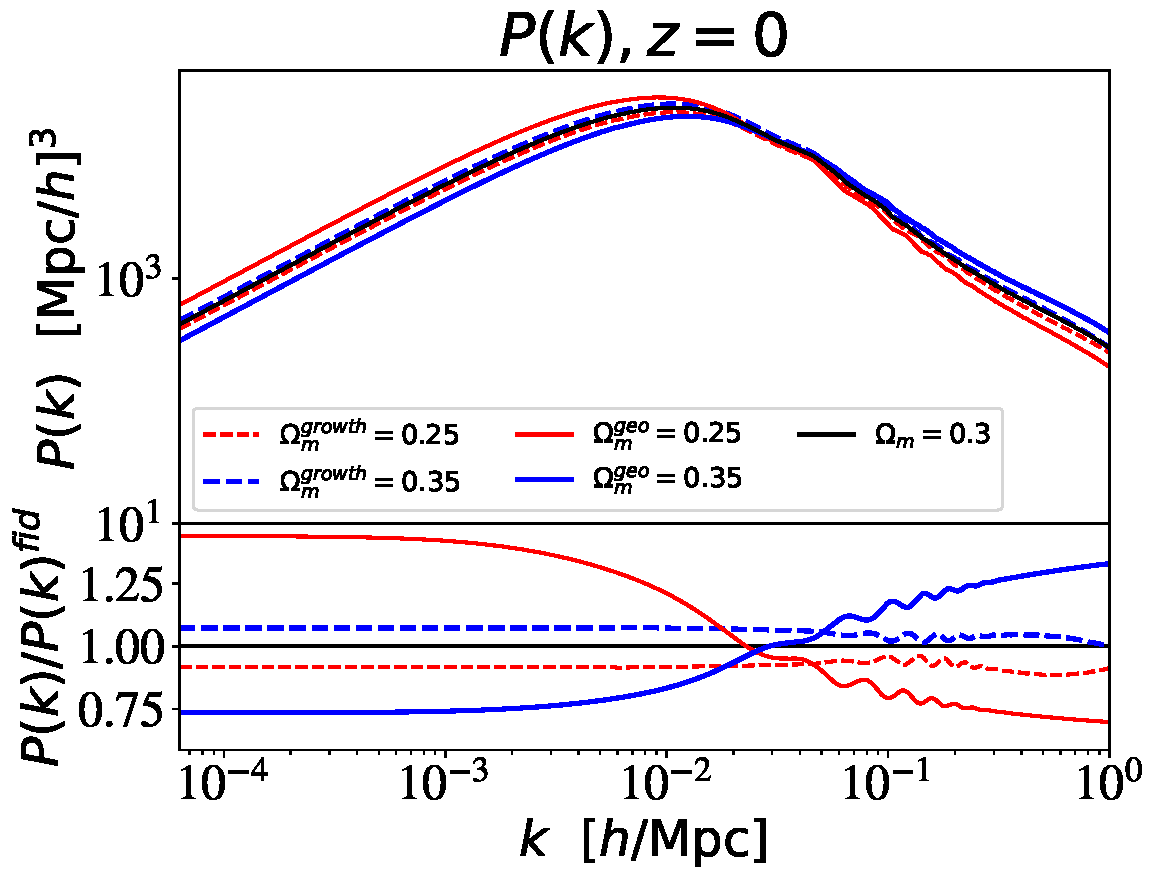
\includegraphics[width=0.75\textwidth]{plots/Pk.pdf}
	\caption{Non-linear power spectrum from Euclid emulator. When either the geometry or growth parameters are varied, the other is kept fixed at $\Omega^X=0.3$.}
	\label{fig:pk}
\end{figure}
While the growth parameters are scale independent, there is a crossing for the geometry parameters. This is due to the enhanced gravitational effects for higher $\Omega_m^{\mathrm{geo}}$, or suppressed gravitational effects for lower $\Omega_m^\mathrm{geo}$. From this, one can predict that the value of $\sigma_8$ will change, the change being larger for $\Omega_m^\mathrm{geo}$ than $\Omega_m^\mathrm{growth}$, and increases in either $\Omega_m$ will increase $\sigma_8$. We see this is true in figure~\ref{fig:sigma8_l}
\begin{figure}[ht]
	\centering
	\begin{subfigure}[b]{0.49\textwidth}
		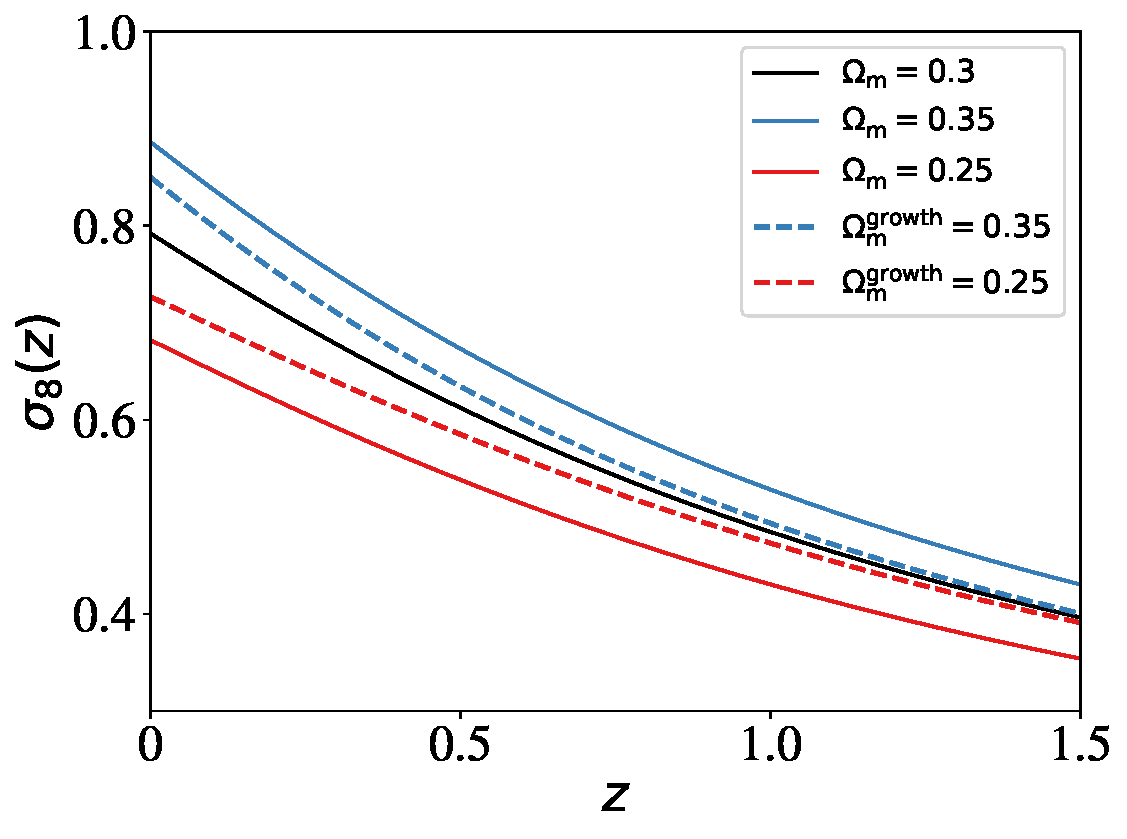
\includegraphics[width=\textwidth]{plots/sigma8.pdf}
		\caption{$\Lambda$CDM split.}
		\label{fig:sigma8_l}
	\end{subfigure}
	\begin{subfigure}[b]{0.49\textwidth}
		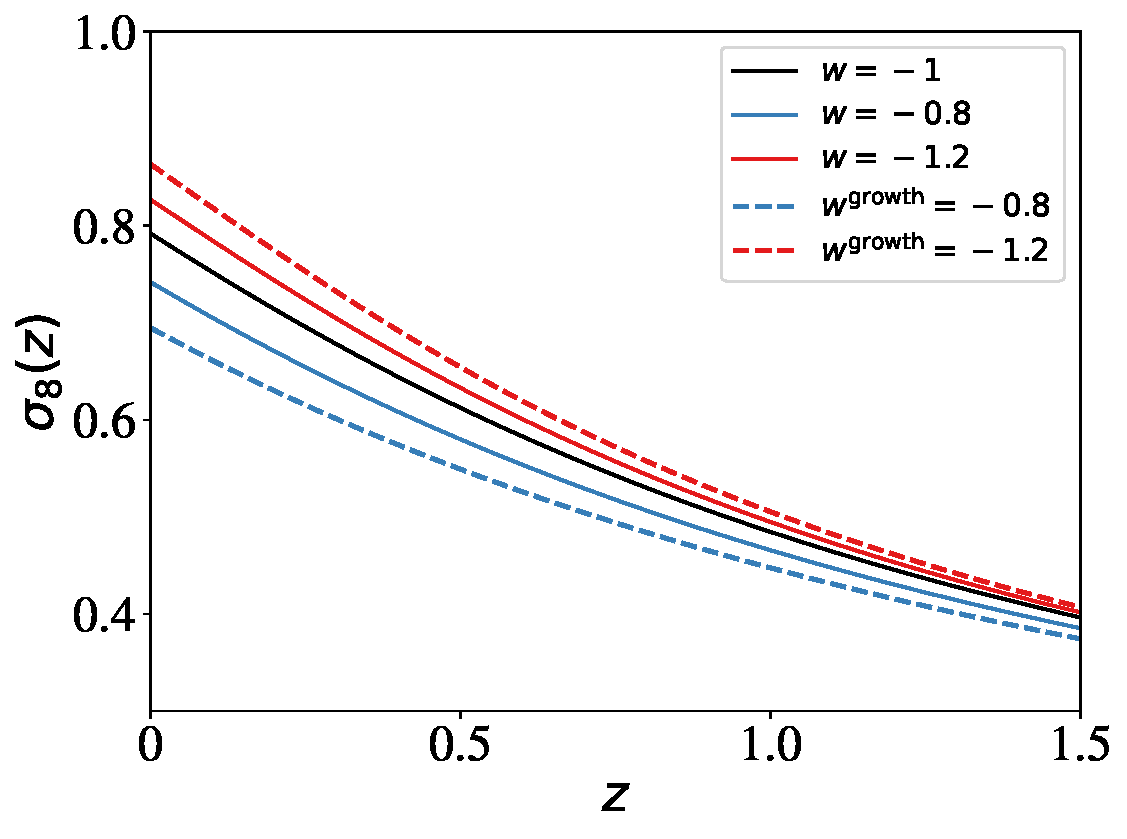
\includegraphics[width=\textwidth]{plots/sigma8_w.pdf}
		\caption{$w$CDM split.}
		\label{fig:sigma8_w}
	\end{subfigure}
	\label{fig:sigma8}
	\caption{Effect of changing growth and geometry parameters on $\sigma_8(z)$.}
\end{figure}
One surprising feature of figure~\ref{fig:sigma8_w} is that these effects are the exact opposite. However, this result is not surprising. Increasing $w$, where $w<0$, coincides with decreasing the pressure or increasing density.
\section{Data and Analysis Pipeline}
\subsection{DES Parameter Priors}
This analysis is done on data from the Dark Energy Survey (DES), both year 1 (Y1) and year 3 (Y3), combined with CMB data. The cosmological parameters of interest and there priors are given in table~\ref{table:cosmo_prior}.
\begin{table}
\centering
\begin{tabular}{lr}
	\hline
	parameter & prior \\
	\hline\hline
	$\Omega_m^{\text{geo}}$    & $\mathcal{U}(0.1,0.9)$   \\
	$w^{\mathrm{geo}}$         & $\mathcal{U}(-3,-0.01)$  \\
	$\mathcal{A}_s\times10^9$  & $\mathcal{U}(1.7,2.5)$   \\
	$n_s$                      & $\mathcal{U}(0.92,1.0)$  \\
	$H_0$                      & $\mathcal{U}(61,73)$     \\
	$\tau$                     & $\mathcal{U}(0.01,0.8)$  \\
	$\Omega_m^{\text{growth}}$ & $\mathcal{U}(0.24,0.4)$  \\
	$w^{\mathrm{growth}}$      & $\mathcal{U}(-1.7,-0.7)$ \\
	\hline
\end{tabular}
\caption{Summary of cosmological parameters and their priors.}
\label{table:cosmo_prior}
\end{table}
The priors on ($\Omega_m^{\text{geo}}$, $w^{\mathrm{geo}}$, $\mathcal{A}_s\times10^9$, $n_s$, $H_0$) are taken from the Euclid Emulator prior. $\tau$ is only included in chains that also contain CMB data.
\begin{table}
\centering
\begin{tabular}{lcc} % 
\hline
DES Systematics Parameter &  Y1 Prior & Y3 Prior \\
\hline\hline
\textbf{Linear Galaxy bias} \\
$ b_g^i(i \in [1,5])$ & Flat(0.8, 3.0) & Flat(0.8, 3.0)\\
\hline
\textbf{Intrinsic Alignment (NLA)} \\
$A_{1}$ &  Flat(-5, 5) & \\
$A_{2}$ &  Flat(-5, 5) & \\
\hline
\textbf{Intrinsic Alignment (TATT)} \\
$A_{1}$    & & Flat(-5, 5) \\
$A_{2}$    & & Flat(-5, 5) \\
$\eta_{1}$ & & Flat(-5, 5) \\
$\eta_{2}$ & & Flat(-5, 5) \\
$b_{TA}$   & & Flat(0 , 2) \\
\hline
\textbf{Source photo-z} \\
$\Delta z_{\mathrm{s}}^{1} \times 10^{2}$ & Gauss(-0.1, 1.6)  & Gauss(0, 1.8) \\
$\Delta z_{\mathrm{s}}^{2} \times 10^{2}$ & Gauss(-0.19, 1.3) & Gauss(0, 1.5) \\
$\Delta z_{\mathrm{s}}^{3} \times 10^{2}$ & Gauss(0.9, 1.1)   & Gauss(0, 1.1)\\
$\Delta z_{\mathrm{s}}^{4} \times 10^{2}$ & Gauss(-1.8, 2.2)  & Gauss(0, 1.7)\\
\hline
\textbf{Lens photo-z}\\
$\Delta z_{\mathrm{1}}^{1} \times 10^{2}$ & Gauss(0.8, 0.7)  & Gauss(0.6, 0.4)  \\
$\Delta z_{\mathrm{1}}^{2} \times 10^{2}$ & Gauss(-0.5, 0.7) & Gauss(0.1, 0.3)  \\
$\Delta z_{\mathrm{1}}^{3} \times 10^{2}$ & Gauss(0.6, 0.6)  & Gauss(0.4, 0.3)\\
$\Delta z_{\mathrm{1}}^{4} \times 10^{2}$ & Gauss(0, 0.01)   & Gauss(-0.2, 0.5)\\
$\Delta z_{\mathrm{1}}^{5} \times 10^{2}$ & Gauss(0, 0.01)  & Gauss(-0.7, 0.1)\\
\hline
\textbf{Multiplicative shear calibration} \\
$m_{1} \times 10^2$ & Gauss(1.2, 2.3) & Gauss(-0.6, 0.9)\\
$m_{2} \times 10^2$ & Gauss(1.2, 2.3) & Gauss(-2.0, 0.8)\\
$m_{3} \times 10^2$ & Gauss(1.2, 2.3) & Gauss(-2.4, 0.8)\\
$m_{4} \times 10^2$ & Gauss(1.2, 2.3) & Gauss(-3.7, 0.8)\\
\hline
\textbf{Lens magnification} \\
$C_{\mathrm{1}}^1 \times 10^2$ & & Fixed (0.63)\\
$C_{\mathrm{1}}^2 \times 10^2$ & & Fixed (-3.04)\\
$C_{\mathrm{1}}^3 \times 10^2$ & & Fixed (-1.33)\\
$C_{\mathrm{1}}^4 \times 10^2$ & & Fixed (2.50)\\
$C_{\mathrm{1}}^5 \times 10^2$ & & Fixed (1.93)\\
\hline
\textbf{Point mass marginalization} \\
$B_i(i \in [1,5])$ & & Flat(-5, 5) \\
\hline
\end{tabular}
\caption{Summary of Priors on DES-Y1 and DES-Y3 systematics parameters.}
\label{table:prior_choices}
\end{table}
The external data sets used are
\begin{itemize}
	\item CMBP: The Planck CMB TTTEEE power spectra together with the non-linear low-$\ell$ EE power spectrum. The spectra are truncated after the first peak ($35<\ell<396$). This mitigates CMB lensing effects, which affect small-scale anisotropies. It also minimizes the late time Integrated Sachs Wolfe effect, which also has a larger effect on small scales.
	\item SNIa: Pantheon Type Ia supernova. As a distance probe, this prior constrains geometry parameters. There are growth effects that we choose not to model at this point, namely the peculiar velocity distributions of supernovae.
	\item BBN: We use a derived constraint on $100\Omega_bh^2$ from Big Bang Nucleosynthesis as
	\item BAO: BAO data is taken from the SDSS DR7 main galaxy sample, the 6dF galaxy survey, and the combined SDSS BOSS DR12 low-$z$ and CMASS galaxy samples. Again, as a distance probe, this is taken as geometry information.
\end{itemize}
To understand these choices of priors, we consider the following combinations:
\begin{itemize}
	\item Prior 1 (P1): Emulator prior + CMBP
	\item Prior 2 (P2): Emulator prior + SNIa + BBN + BAO
	\item Prior 3 (ALL): Emulator prior + CMBP + SNIa + BBN + BAO
\end{itemize}
\subsection{Software Pipeline}
To compute the linear matter power spectrum we use \textsc{CAMB} Boltzmann code, which is capable of solving the linear Boltzmann equation and computing transfer functions. For going beyond linear scales, we use the Euclid emulator, a fast neural network based emulator for Halofit. Previous DES studies used Halofit itself, a full N-body simulation to determine the non-linear evolution of dark matter. A baseline comparison between the Euclid emulator and Halofit was done (figure~\ref{fig:euc_v_halo})
\begin{figure}[ht]
	\centering
	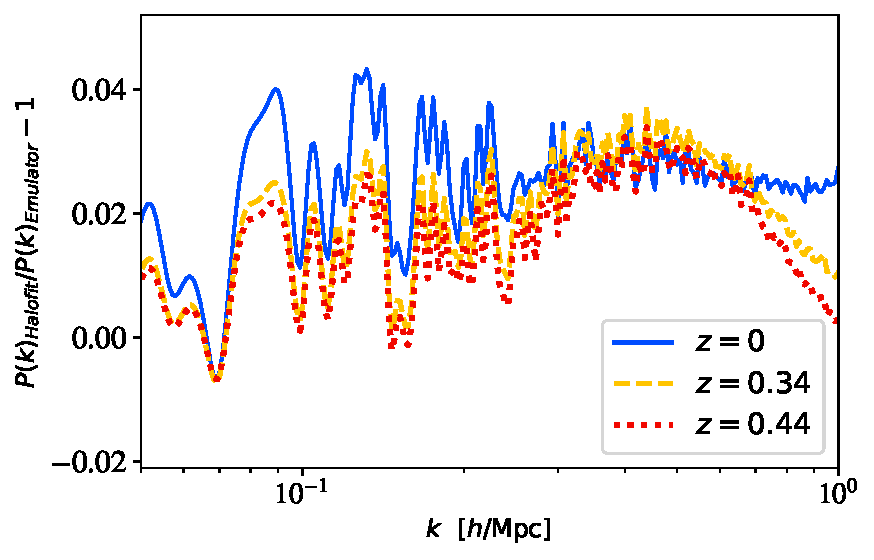
\includegraphics[width=0.75\textwidth]{plots/halo_vs_emu.pdf}
	\caption{Relative difference between Euclid emulator and Halofit.}
	\label{fig:euc_v_halo}
\end{figure}
We use the Cocoa (CObaya-COsmolike joint Architecture). This interfaces Cobaya, the MCMC sampler we use, with Cosmolike, the data vector calculation framework. DES-Y3 has already been implemented in Cobaya, Cosmolike, and Cocoa. To assess the convergence of the MCMC, we use the $R-1<0.02$.

One benefit of this analysis is that growth parameters are semi-fast; they do not require CAMB to recompute the matter power spectrum, they only require Cosmolike to update the data vectors. Rerunning Cosmolike with only changing the growth parameters results in a 2-fold speedup.
\subsection{Pipeline Validation on Synthetic Data}
To validate this method, we generate a synthetic data vector at the Planck best-fit parameters without lensing (equation~\ref{eq:planck_best_fit}), and we hope to find no difference between growth and geometry parameters and hope each parameter is equal to the fiducial value.
\begin{equation}\label{eq:planck_best_fit}
	(\mathcal{A}_s\times10^{-9}, n_s, H_0, \Omega_m, \Omega_b) = (2.101,0.965,67.32,0.317,0.049)
\end{equation}
Using the ALL prior and external data, there is marginal improvement between the cosmic shear constraints on $\Omega_m^\mathrm{growth}$ compared to the prior. However there is significant improvement in the 3x2pt case compared to cosmic shear. 

The constraining power of 3x2pt on $\Omega_m^\mathrm{growth}$ is identical between P1 and ALL. This is because ...

In $w$CDM, there is poor constraining power on $\Omega_m^\mathrm{growth}$ and $w^{\mathrm{growth}}$, even with the most informative 3x2pt case. For this case, we give constraining power along the first principle component
\begin{equation}
	\mathrm{PC}_1 \equiv 0.7071\Delta\Omega_m - 0.7071\Delta w\,.
\end{equation}
In all 3 sets of priors and external data, and despite the inclusion of additional nuisance parameters from the TATT model, we find similar constraining power on $\Omega_m^\mathrm{growth}$ between DES-Y1 and DES-Y3. In the 3x2pt case with the ALL prior gives a smaller ($\sim17\%$) error bar. Constraints on $\mathrm{PC}_1$ are prior dominated and nearly identical for the $w$CDM split in DES-Y1 and DES-Y3.
\begin{figure}[ht]
	\centering
	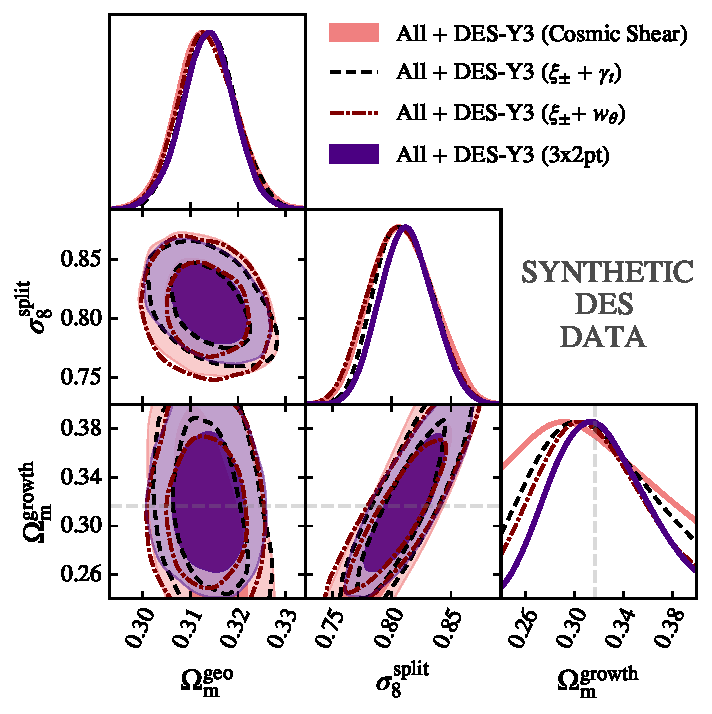
\includegraphics[width=0.75\textwidth]{plots/plot36_S8.pdf}
	\caption{Cosmic shear, 2x2pt combinations, and 3x2pt posteriors for DES-Y3 with the ALL prior.}
	\label{fig:syn_y3_probe}
\end{figure}
\begin{figure}[ht]
	\centering
	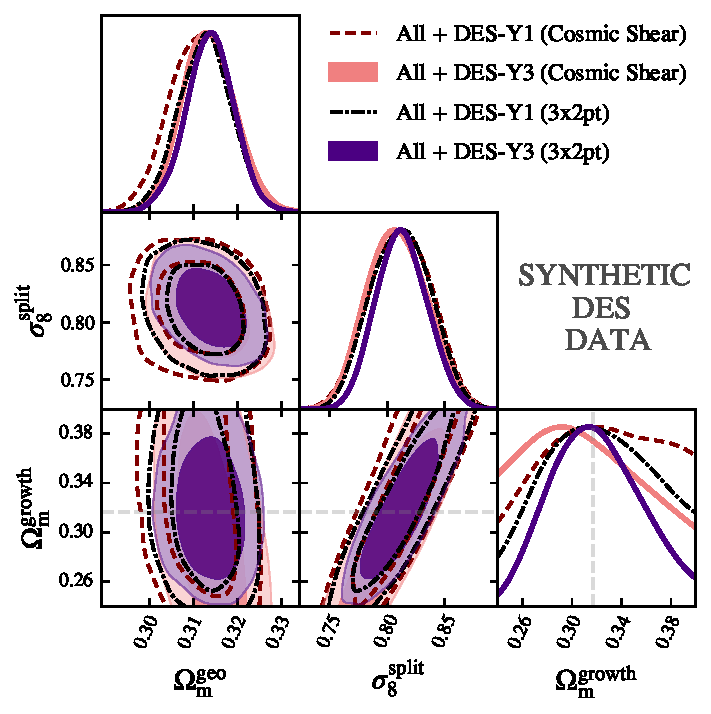
\includegraphics[width=0.75\textwidth]{plots/plot31v3.pdf}
	\caption{Comparison of DES-Y1 and DES-Y3 posteriors.}
	\label{fig:syn_y1_y3}
\end{figure}
\section{Results}
\subsection{LCDM}
For the most constraining case, 3x2pt with all prior, there is no evidence of a difference between $\Omega_m$ growth and geometry parameters (figure~\ref{fig:y3_3x2_all}). Exploring this further, however, we can look at various 2-point correlation functions is DES-Y1 and DES-Y3 (figure~\ref{fig:y3_2x2}). We see a significant change in the DES-Y3 cosmic shear-galaxy clustering posterior and the galaxy lensing-galaxy clustering posterior. However, these shifts from $\Delta\Omega_m=0$ are prior dominated, not data dominated, thus do not constitute evidence for a shift.
\begin{figure}[ht]
	\centering
	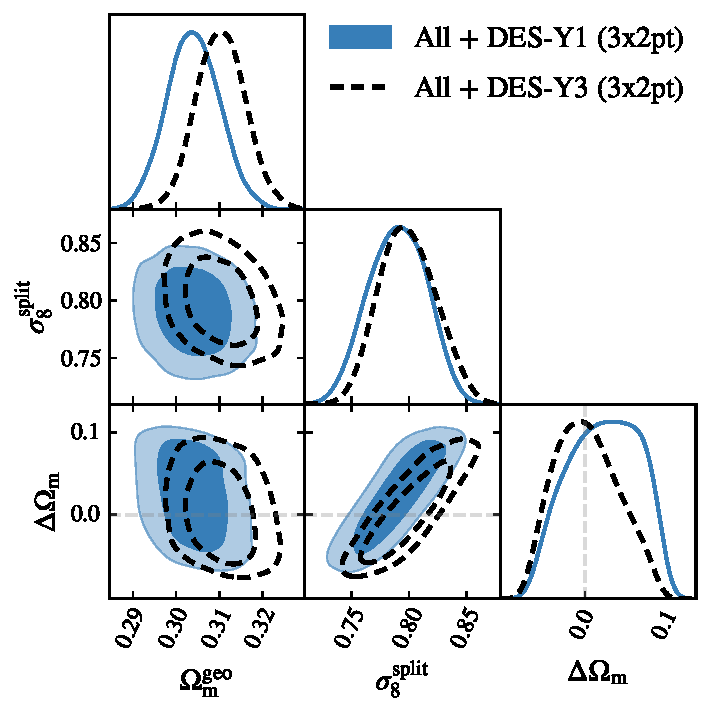
\includegraphics[width=0.75\textwidth]{plots/plot204_v2.pdf}
	\caption{Split posteriors for DES-Y3 3x2pt and ALL prior.}
	\label{fig:y3_3x2_all}
\end{figure}
\begin{figure}[ht]
	\centering
	\begin{subfigure}[b]{0.45\textwidth}
		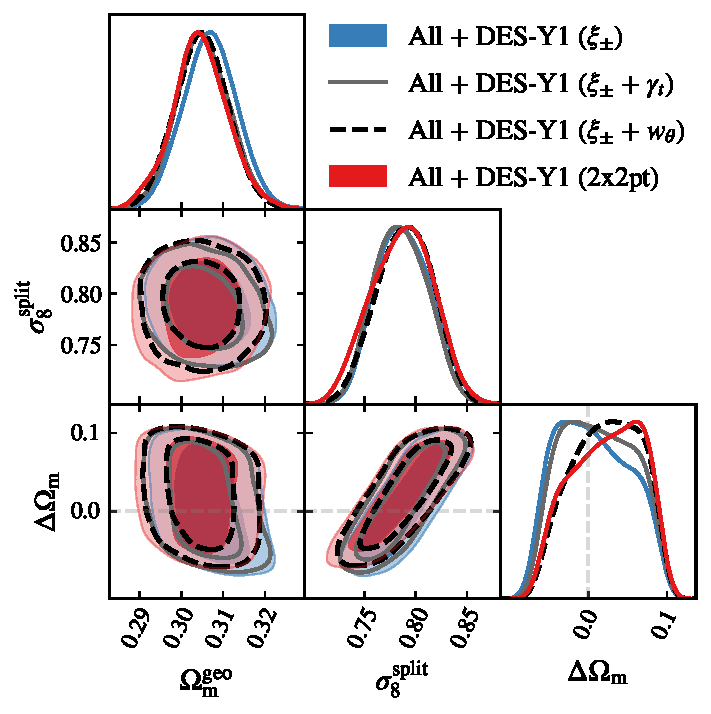
\includegraphics[width=\textwidth]{plots/plot208_v3.pdf}
		\caption{DES-Y1}
		\label{fig:y1_2x2_lcdm}
	\end{subfigure}
	\begin{subfigure}[b]{0.45\textwidth}
		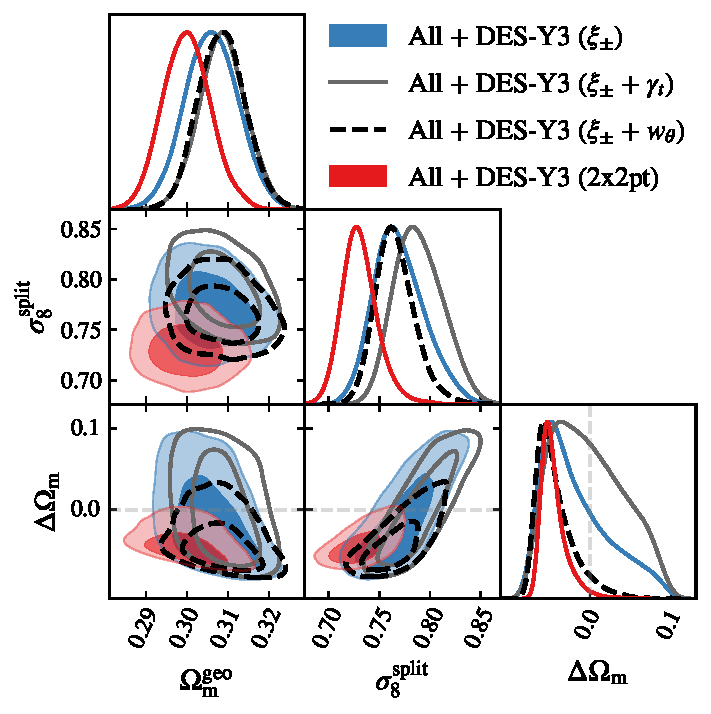
\includegraphics[width=\textwidth]{plots/plot208_v2.pdf}
		\caption{DES-Y3}
		\label{fig:y3_2x2_lcdm}
	\end{subfigure}
	\caption{DES-Y1 and DES-Y3 posteriors for 2-point correlation functions.}
	\label{fig:y3_2x2}
\end{figure}
The full results of the 1d marginalizations with each choice of prior is summarized in figure~\ref{fig:lcdm_result_1d}. Aside from the previously mention 2-point correlation functions, every $\Delta\Omega_m$ result is compatible with 0 to within 1-sigma.
\begin{figure}[ht]
	\centering
	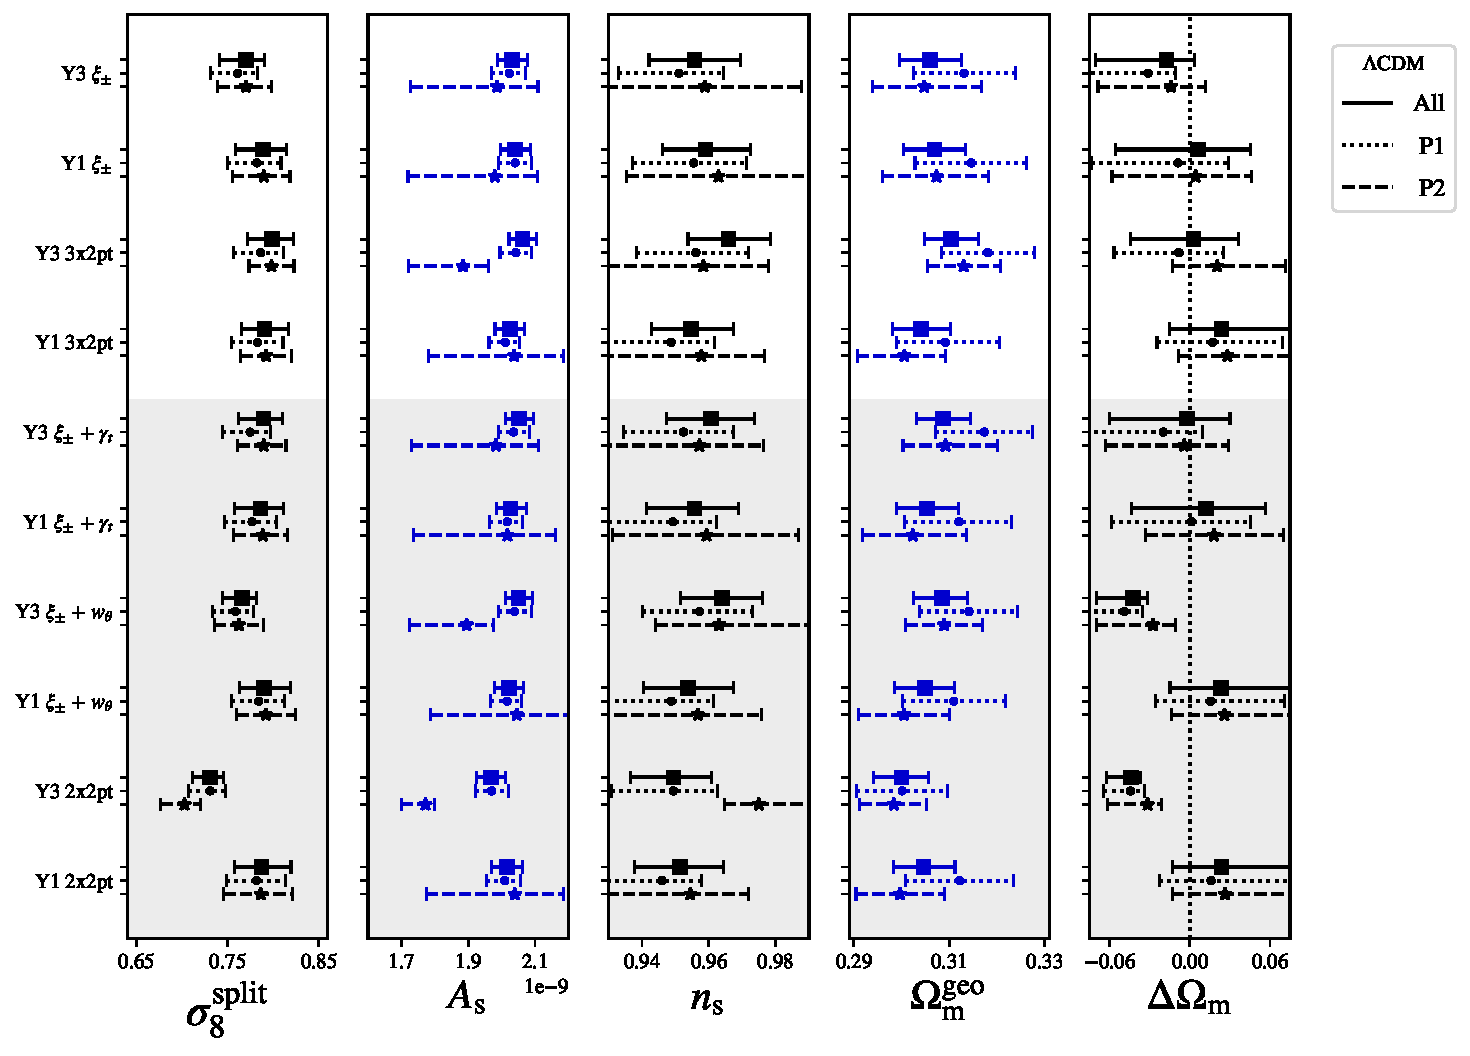
\includegraphics[width=\textwidth]{plots/plot_1d_resultv5.pdf}
	\caption{Full 1d results for $\Lambda$CDM split}
	\label{fig:lcdm_result_1d}
\end{figure}
Similarly to the synthetic chains, the 3x2pt data chains with ALL prior have improved constraining power on $\Delta\Omega_m$ in DES-Y3 over DES-Y1. However, the improvement is around 10\%, slightly less than the 17\% observed in the synthetic data. 

The mentioned 2-point correlation functions that do have significant shifts in $\Omega_m$ are determined to be at $1.75\sigma$ for the cosmic shear-galaxy clustering and $2.60\sigma$ for galaxy clustering-galaxy-galaxy lensing. Because of known inconsistencies in the RedMaGiC galaxy samples, these are not attributed to discovery.
\subsection{wCDM}
The results for $w$CDM are summarized in figures~\ref{fig:wcdm_post} and~\ref{fig:wcdm_result_1d}. Again, there is no evidence of a shift in $\mathrm{PC}_1$ from 0. The exception is, once again, the DES-Y3 2x2pt with ALL prior. The significance of the shift is $4.48\sigma$. Again, this shift may be attributed to the RedMaGiC. 
\begin{figure}[ht]
	\centering
	\begin{subfigure}[b]{0.45\textwidth}
		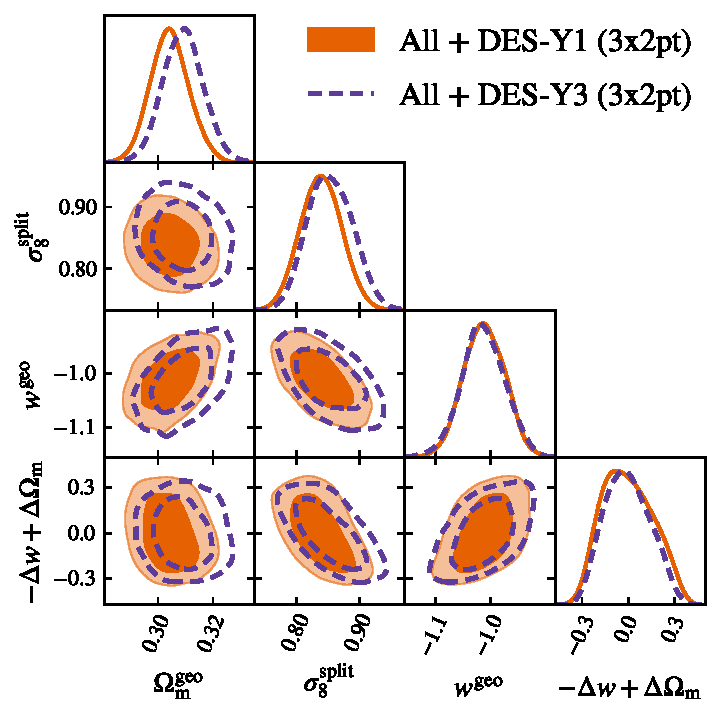
\includegraphics[width=\textwidth]{plots/plot205v2.pdf}
		\caption{DES-Y1 vs DES-Y3 3x2pt $w$CDM posteriors.}
		\label{fig:y3_y1_wcdm}
	\end{subfigure}
	\begin{subfigure}[b]{0.45\textwidth}
		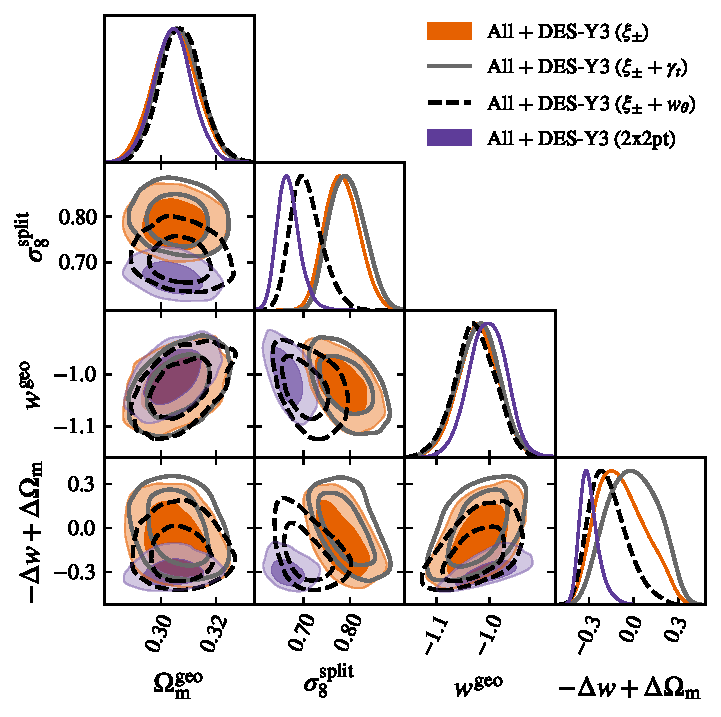
\includegraphics[width=\textwidth]{plots/plot209.pdf}
		\caption{DES-Y3 2-point correlation function posteriors}
		\label{fig:y3_2x2_wcdm}
	\end{subfigure}
	\caption{$w$CDM posteriors.}
	\label{fig:wcdm_post}
\end{figure}
\begin{figure}[ht]
	\centering
	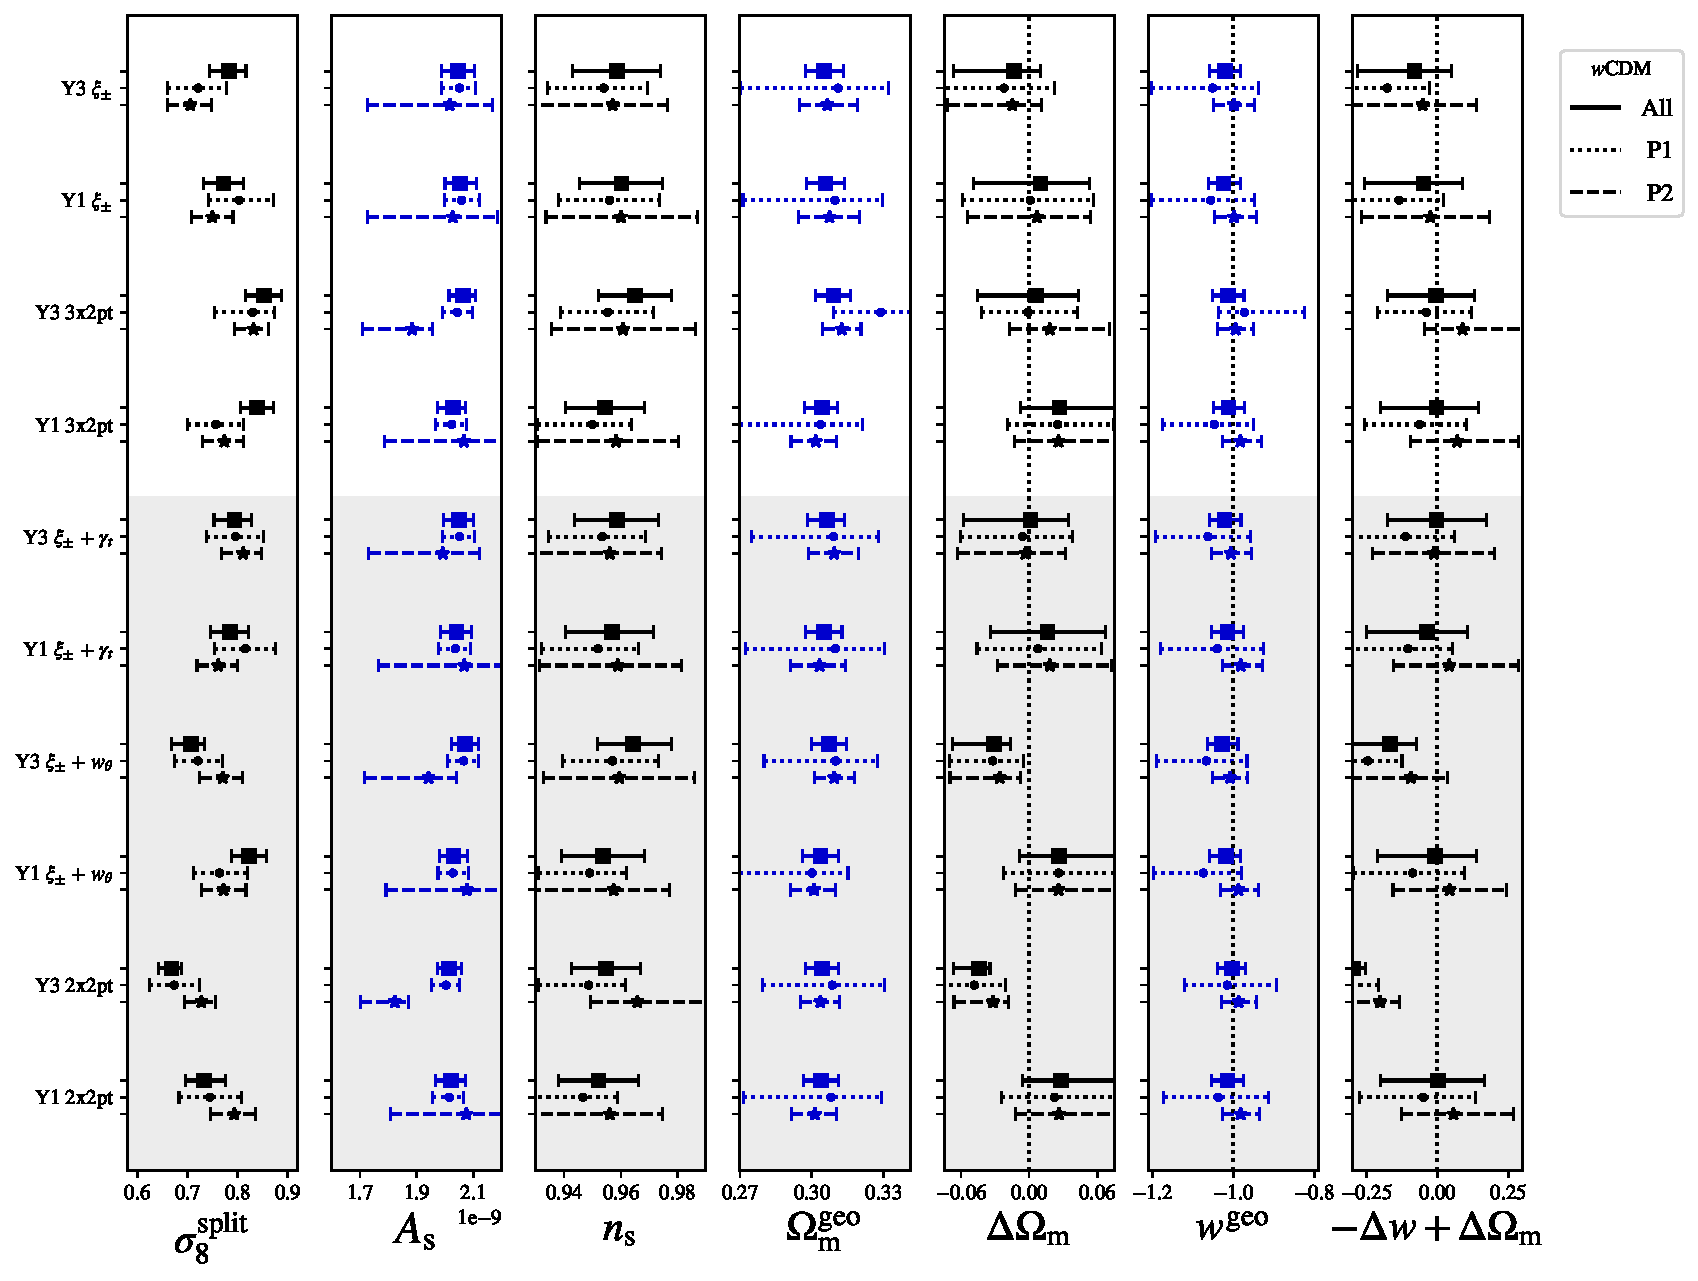
\includegraphics[width=\textwidth]{plots/plot_1d_resultv6.pdf}
	\caption{Full 1d results for $\Lambda$CDM split}
	\label{fig:wcdm_result_1d}
\end{figure}
\subsection{Tension Analysis}
We conclude by testing the internal consistency between the Y1 and Y3 data sets independently. This is done using the parameter difference method, where we use normalizing flows to learn the posterior distribution. The results are summarized in figure~\ref{fig:tension}. The tension is computed with the parameters $(\mathcal{A}_s,n_s,H_0,\Omega_m^{\mathrm{geo}},\sigma_8^\mathrm{split})$ (with $w^{\mathrm{geo}}$ added in the $w$CDM case). Interestingly, the tension appears to be generated predominantly by $\mathcal{A}_s$. Additionally, the 2x2pt correlation functions have a significant degradation in the goodness of fit when CMB priors are added. This reflects the RedMaGiC inconsistency discussed above. A study allowing $X_\mathrm{lens}$ to vary is required to fully analyze this shift.

In the $w$CDM case, we once again see the 2x2pt has a significant shift. Contrary to the split $\Lambda$CDM case, the $\mathcal{A}_s$ tension is much smaller, making the detection of a shift in $\mathrm{PC}_1$ more meaningful. Once again, an analysis involving $X_\mathrm{lens}$ is required to assess the source of this detection.
\begin{figure}[ht]
	\centering
	\begin{subfigure}[b]{0.45\textwidth}
		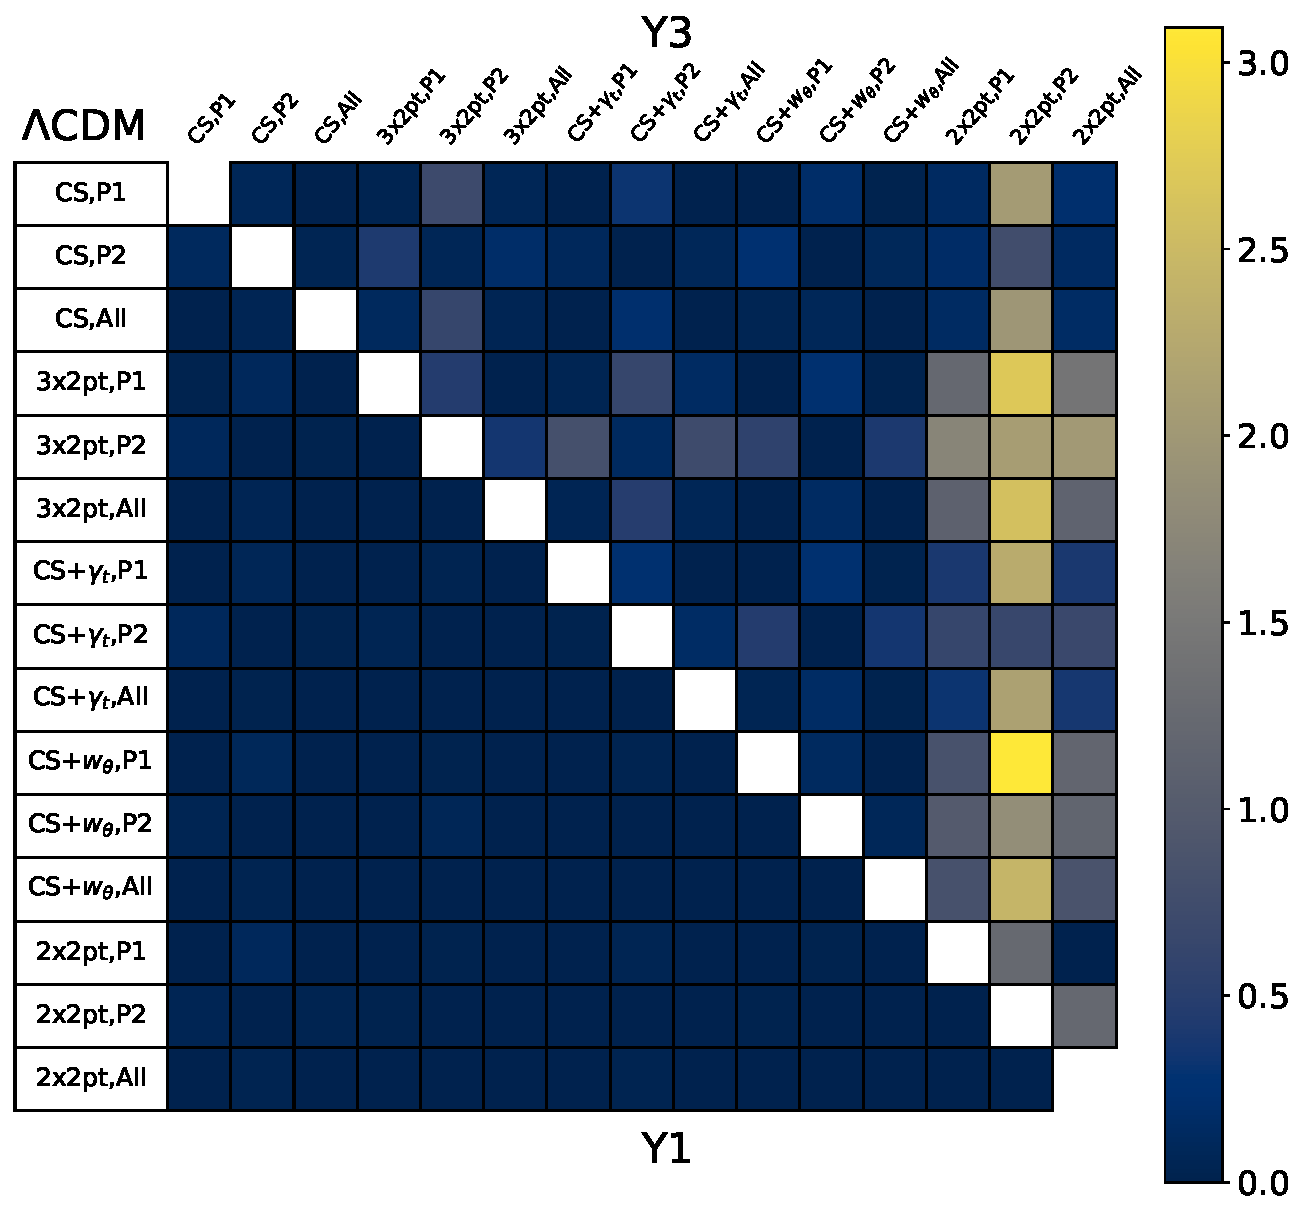
\includegraphics[width=\textwidth]{plots/internal_tension_v4.pdf}
		\caption{Internal tension in the $\Lambda$CDM split.}
		\label{fig:lcdm_tension}
	\end{subfigure}
	\begin{subfigure}[b]{0.45\textwidth}
		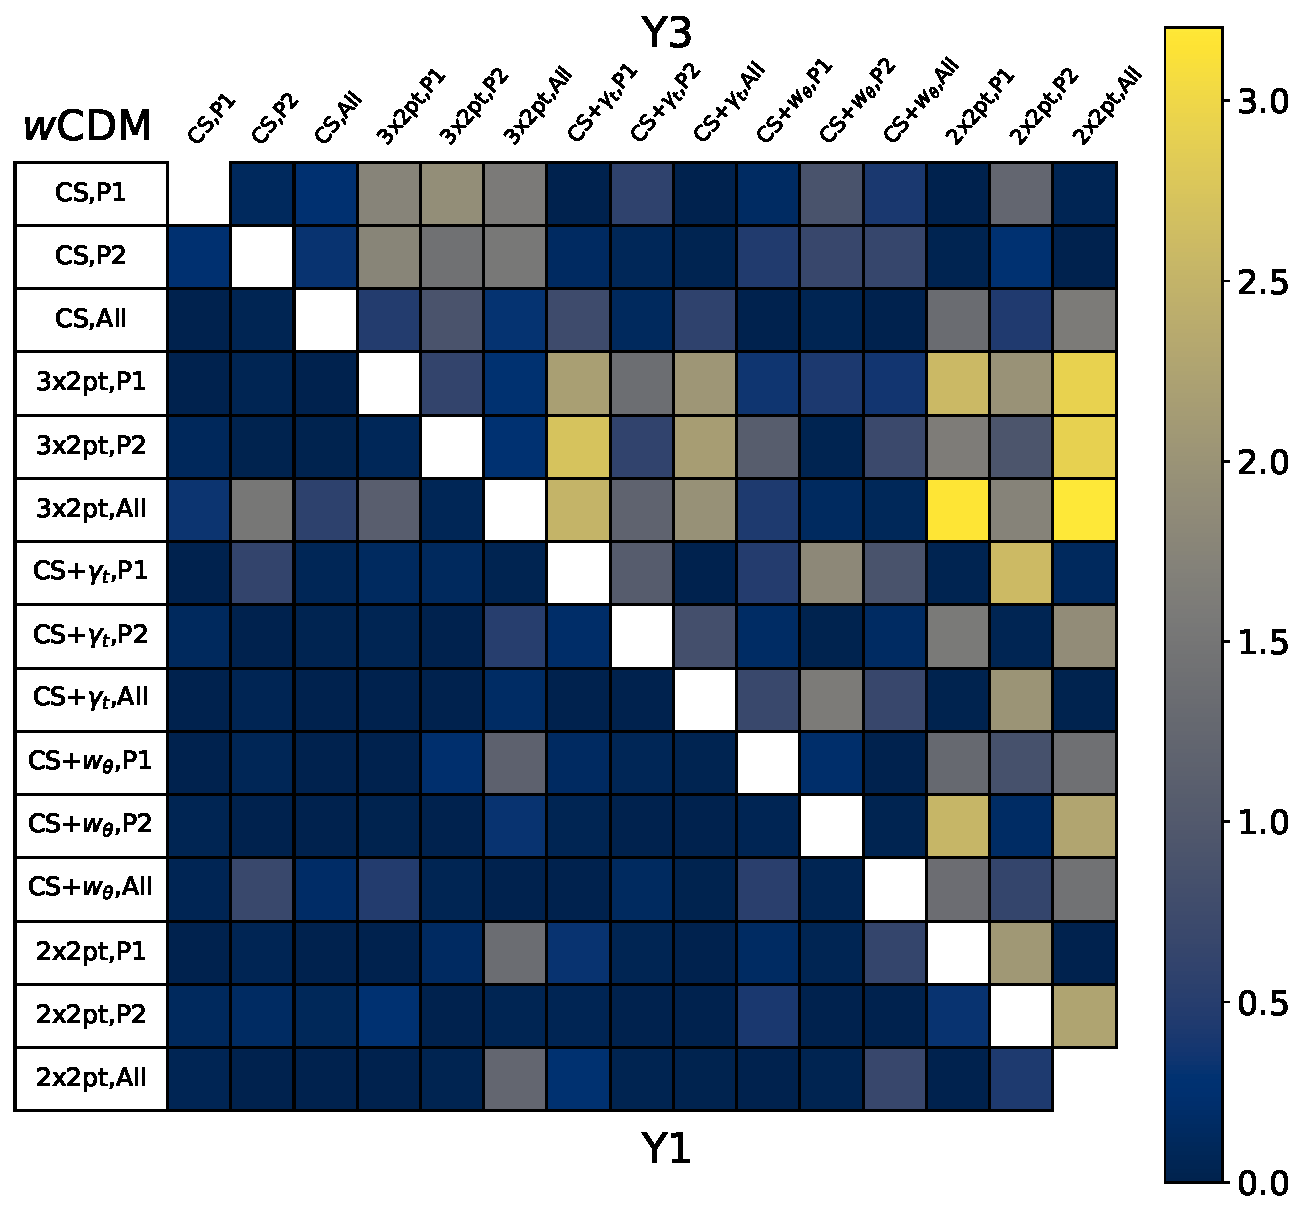
\includegraphics[width=\textwidth]{plots/internal_tension_wcdm.pdf}
		\caption{Internal tension in the $w$CDM split}
		\label{fig:wcdm_tension}
	\end{subfigure}
	\caption{}
	\label{fig:tension}
\end{figure}
\section{Conclusion}
We split $\Omega_m$ and $w$ into two parameters, one governing the background evolution and the other governing the late-time scale-independent growth of structure. We consider DES data together with various external data sets and priors from the CMB, supernovae, BBN, and BAO. We then run MCMC on DES-Y1 and DES-Y3 data and evaluate the difference between the growth and geometry parameters. 

As demonstrated, there is little evidence of a difference between growth and geometry parameters in DES-Y1 and DES-Y3. The exception is the 2x2pt chains, however there is an internal inconsistency with the RedMaGiC samples that may source this result. Because we fixed $X_\mathrm{lens}=1$, an additional analysis can be done investigating if $X_{\mathrm{lens}}$ sources significant shift. Additionally, one can repeat the analysis with the MagLim lensing samples. In the future, additional datasets from Rubin Observatory's LSST, the Euclid mission, Dark Energy Spectroscopic Instrument, Simons Observatory, and CMB-S4 can be used to improve the constraints derived in this analysis
